\chapter{PX4 autopilot}

PX4 je profesionální autopilot, vyvinutý světovými vývojáři z průmyslu a akademické obce a podporovaný aktivní celosvětovou komunitou. Pohání všechny druhy vozidel od závodních a nákladních dronů až po pozemní vozidla a ponorky. 

\section{Architektura PX4}

PX4 firmware se skládá ze dvou hlavních vrstev:
\begin{itemize}
    \item Flight stack (letový zásobník)
    \begin{itemize}
        \item Letový zásobník je systém pro odhad a řízení letu.
    \end{itemize}
    \item PX4 middleware
    \begin{itemize}
        \item PX4 middleware je obecná robotická vrstva, která podporuje jakýkoli typ autonomního robota a poskytuje interní/externí komunikaci a integraci s hardware.
        \item Middleware navíc obsahuje simulační vrstvu, která umožňuje spuštění letového kódu PX4 na desktopovém operačním systému a ovládání počítačem modelovaného vozidla v simulovaném prostoru.\\
    \end{itemize}
\end{itemize}

Všechny podporované typy vozidel (drony, letadla, čluny, rovery, ponorky atd.) sdílejí jedinou kódovou základnu, která má následující vlastnosti: \cite{PX4main}

\begin{itemize}
    \item Veškerá funkčnost je rozdělena na vyměnitelné a opakovaně použitelné komponenty
    \item Komunikace probíhá pomocí asynchronního předávání zpráv
    \item Systém se dokáže vypořádat s různou pracovní zátěží\\
\end{itemize}

Na obrázku \ref{fig:PX4_Arch} je zobrazen diagram, který poskytuje podrobný přehled stavebních bloků PX4. Horní část diagramu obsahuje middlewarové bloky, zatímco spodní část zobrazuje komponenty letového zásobníku (\textit{flight stack}).

Moduly spolu komunikují prostřednictvím sběrnice \textit{publish-subscribe} s názvem \textit{uORB}. Hlavní výhody schématu \textit{publish-subscribe} v PX4 jsou následující:

\begin{itemize}
    \item Systém je asynchronní a aktualizuje se okamžitě, když jsou k dispozici nová data
    \item Všechny operace a komunikace jsou plně paralelní
    \item Systémová komponenta může zpracovávat data odkudkoli (globální datový prostor)
\end{itemize}

\begin{figure}[!ht]
    \begin{center}
        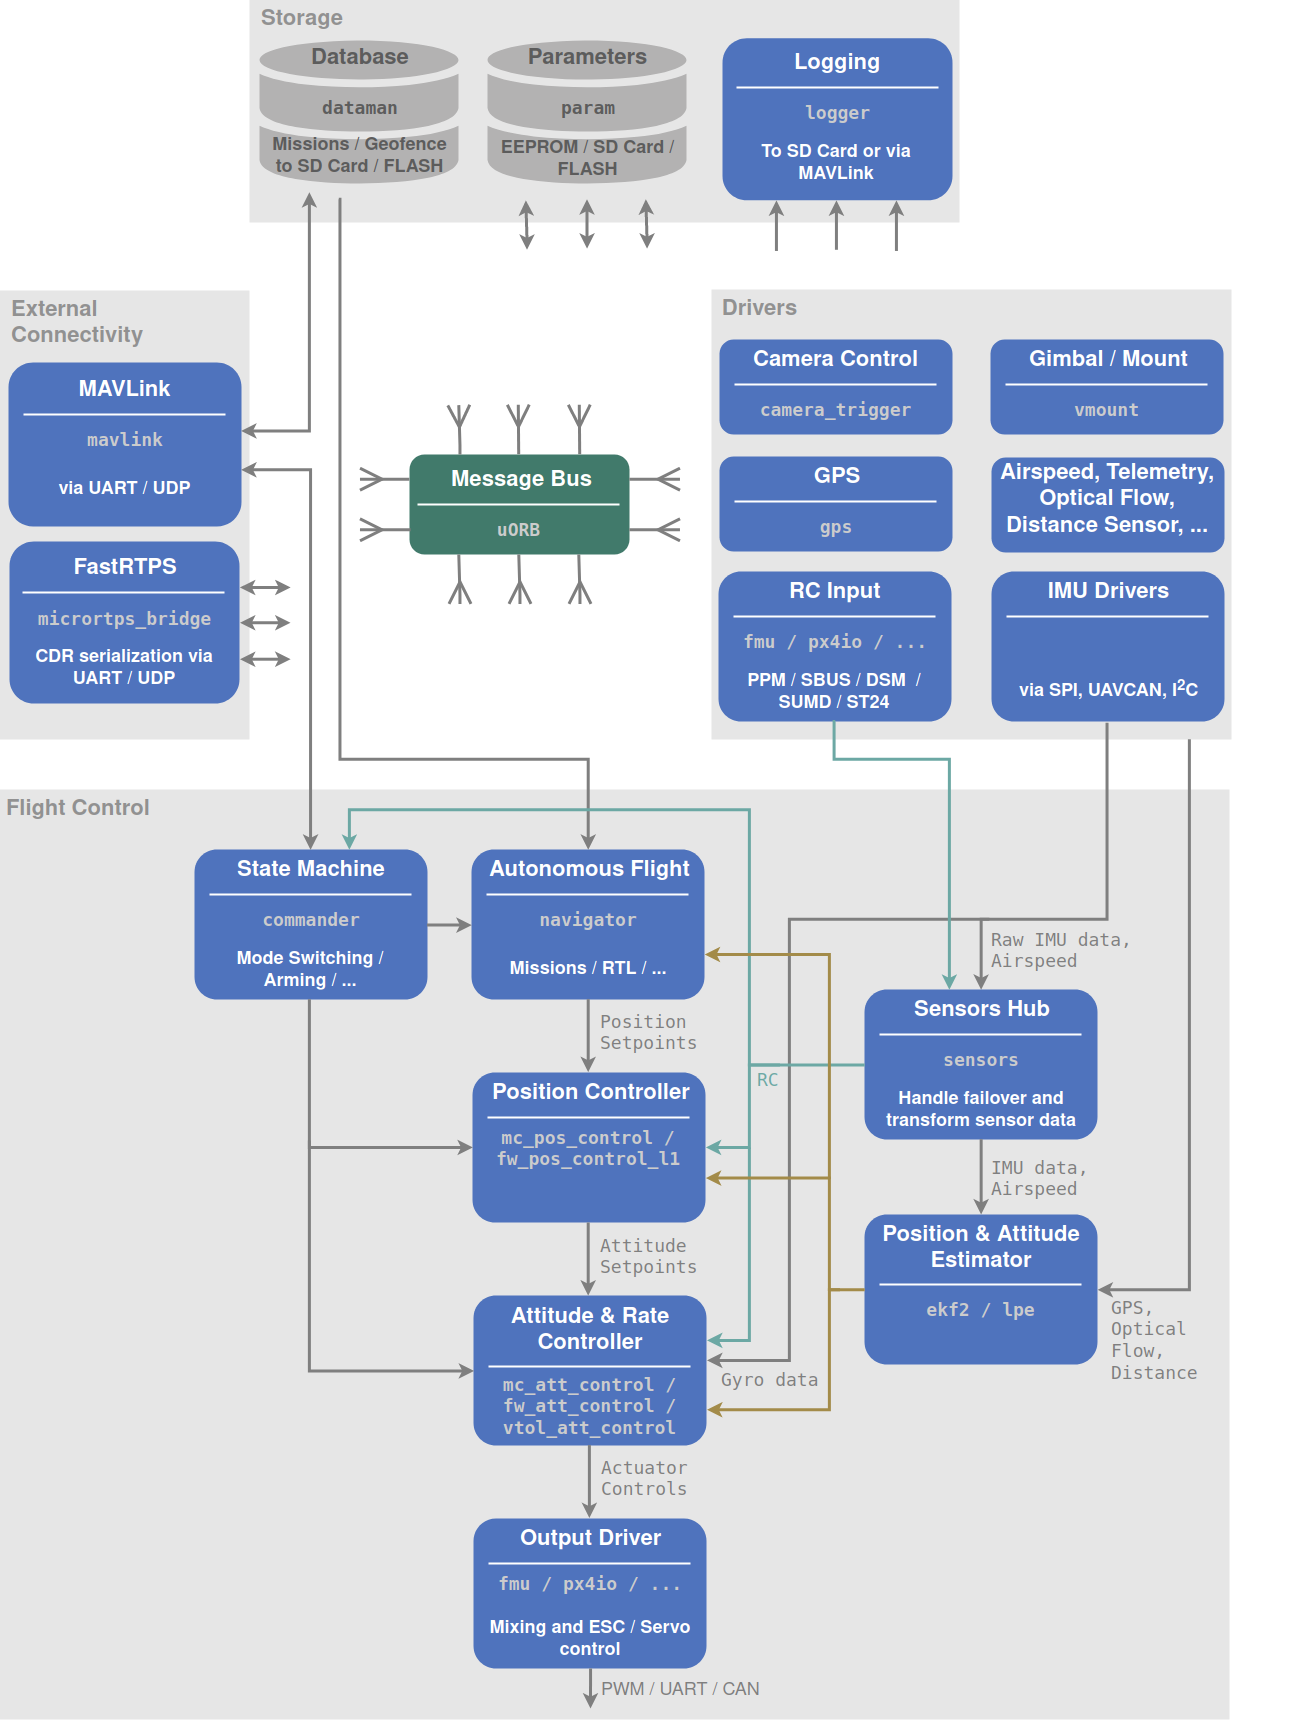
\includegraphics[scale=0.45]{obrazky/PX41}
    \end{center}
    \caption[Komplexní strukturální architektura PX4 software]{Komplexní strukturální architektura PX4 software \cite{PX4main}.}
    \label{fig:PX4_Arch}
\end{figure}

\subsection{PX4 jako samotný letový ovladač}

Na obrázku \ref{fig:PX4_FC} je naznačená architektura systému založeného na letovém ovladači (řídící jednotce) (\textit{flight controller}). Řídící jednotka zabezpečuje sběr dat ze senzorů, ovládání akčních členů dronu (pohony, serva, ...), řízení dronu na základě dat ze senzorů a povelů z RC rádia a v neposlední řadě stabilizaci dronu.

Do systému PX4 je možné zasílat povely z pozemní stanice (\textit{Ground Station}) přes protokol \textit{MAVlink} pomocí telemetrické rádiové soupravy.

\begin{figure}[!ht]
    \begin{center}
        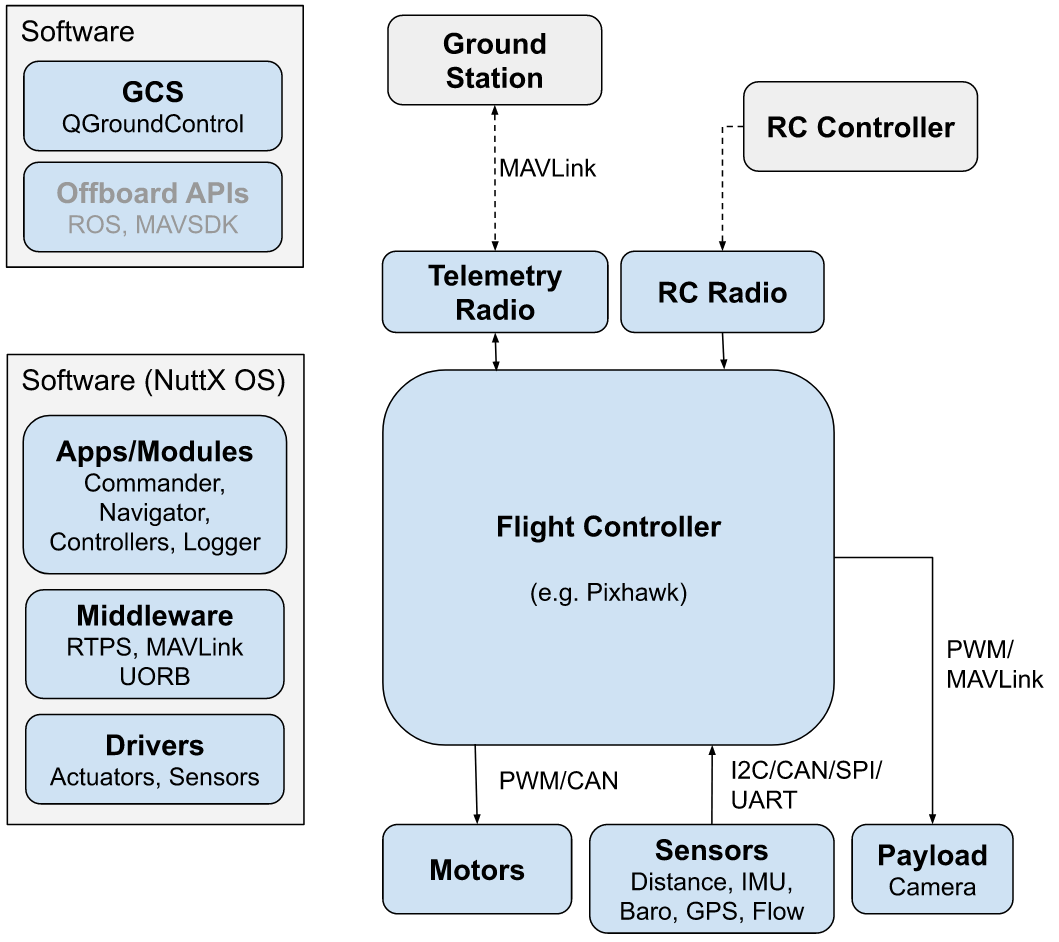
\includegraphics[scale=0.36]{obrazky/PX42}
    \end{center}
    \caption[Jednoduchý systém PX4 založený na letovém ovladači (flight controller)]{Jednoduchý systém PX4 založený na letovém ovladači (flight controller) \cite{PX4main2}.}
    \label{fig:PX4_FC}
\end{figure}

\subsection{Letový ovladač a počítač pro řízení mise}

Na obrázku \ref{fig:PX4_FC_PC} je zobrazená architektura systému PX4 založeného na letovém ovladači (řídící jednotce) a palubním počítači pro řízení mise. Řídící jednotka zabezpečuje sběr dat ze senzorů a ovládání akčních členů dronu (pohony, serva, ...). Komunikace mezi řídící jednotkou zabezpečuje protokol MAVlink, nebo \acs{RTPS} (\acl{RTPS}).

Palubní počítač pro řízení mise poskytuje pokročilé funkce, jako je vyhýbání se objektům a předcházení kolizím. Obvyklým operačním systémem je Linux s ROS (ROS 2) z důvodu, podpory knihoven na předcházení kolizím a z důvodu, že ROS 2 a PX4 využívají pro komunikaci s okolím \acs{DDS} (\acl{DDS}) middleware.

\begin{figure}[!ht]
    \begin{center}
        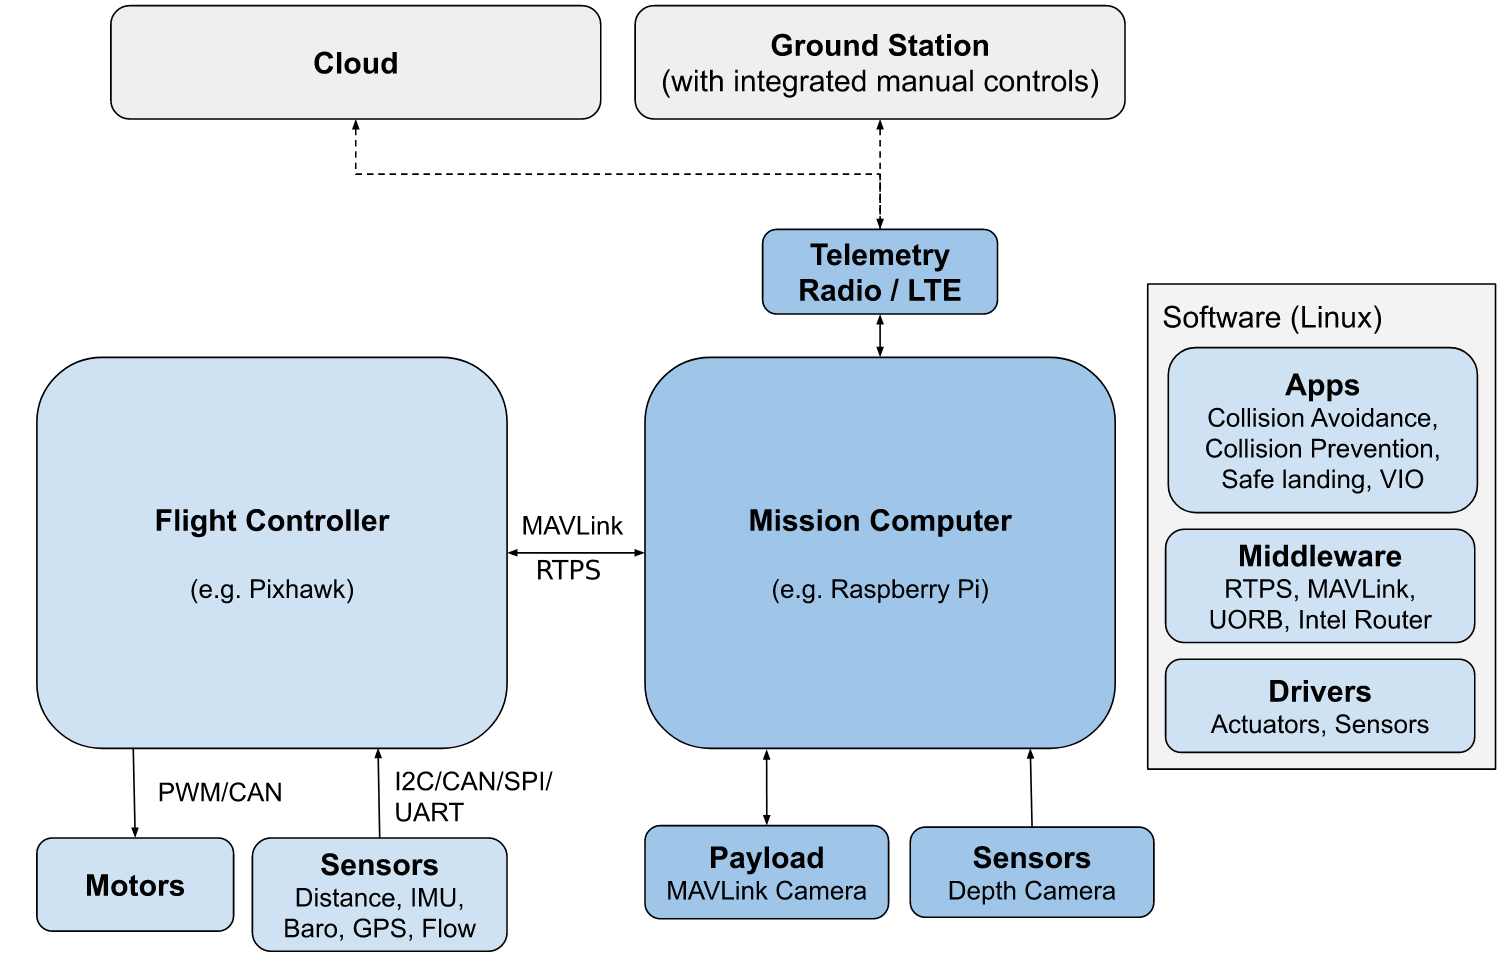
\includegraphics[scale=0.37]{obrazky/PX43}
    \end{center}
    \caption[Systém PX4 založený na letovém ovladači (flight controller) a palubním počítači pro řízení mise]{Systém PX4 založený na letovém ovladači (flight controller) a palubním počítači pro řízení mise \cite{PX4main2}.}
    \label{fig:PX4_FC_PC}
\end{figure}

\section{Licence}

Kód PX4 je zdarma k použití a úpravě za podmínek permisivní licence \textit{BSD 3-clause license} \cite{BSDlicense}.

Redistribuce a použití ve zdrojové a binární formě, s úpravami nebo bez nich, jsou povoleny za předpokladu, že jsou splněny následující podmínky:

1. Redistribuce zdrojového kódu musí obsahovat výše uvedenou poznámku o autorských právech, tento seznam podmínek a následující prohlášení o vyloučení odpovědnosti.

2. Redistribuce v binární formě musí reprodukovat výše uvedenou poznámku o autorských právech, tento seznam podmínek a následující prohlášení o vyloučení odpovědnosti v dokumentaci a/nebo jiných materiálech dodávaných s distribucí.

3. Jméno držitele autorských práv ani jména jeho přispěvatelů nesmí být použita k podpoře nebo propagaci produktů odvozených z tohoto software bez předchozího výslovného písemného povolení.

\section{QGround Control}

QGroundControl je software, který poskytuje plnou kontrolu letu a plánování mise pro jakýkoli dron s podporou MAVLink. Jeho primárním cílem je snadné použití pro profesionální uživatele a vývojáře. Veškerý kód je open source, takže je možné přispívat a dál ho vyvíjet \cite{QGround}.

Pomocí QGroundControl je možné nahrát nejnovější PX4, nebo Ardupilot firmware do letového ovladače (\textit{flight controller}), nastavit typ konstrukce dronu, ladit parametry regulace a vytvářet autonomní mise pomocí waypointů. Veškeré nastavení dronu a misí je jednoduché a velmi intuitivní.

Obrázek \ref{fig:QGC} zobrazuje základní obrazovku software QGroundControl.

\begin{figure}[!ht]
    \begin{center}
        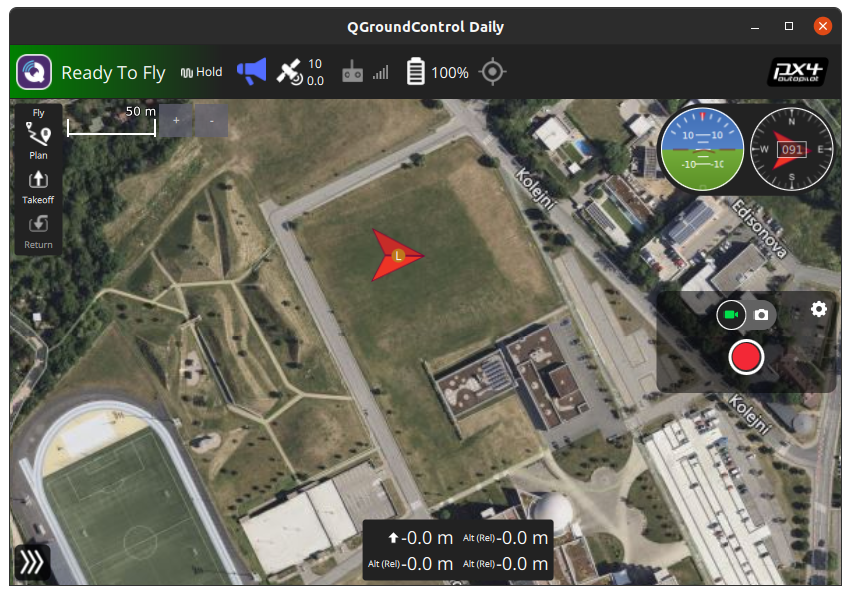
\includegraphics[scale=0.47]{obrazky/QG1}
    \end{center}
    \caption[Základní obrazovka QGroundControl]{Základní obrazovka QGroundControl.}
    \label{fig:QGC}
\end{figure}

Na základní obrazovce jsou zobrazeny stavové informace o dronu:

\begin{itemize}
    \item Relativní výška
    \item Azimut
    \item Orientace dronu (pitch, roll)
    \item RSSI (\textit{Received Signal Strength Indication})
    \item Počet připojených GPS satelitů
    \item Procento nabití akumulátoru
    \item Letový mód
\end{itemize}

\subsection{Nastavení konstrukce dronu}

Systém QGroundControl podporuje velké množství typů konstrukcí dronů, letadel, roverů a ponorek. Obrázek \ref{fig:QGC1} zobrazuje všechny podporované typy zařízení, které dokáže systém PX4 ovládat.

\begin{figure}[!ht]
    \begin{center}
        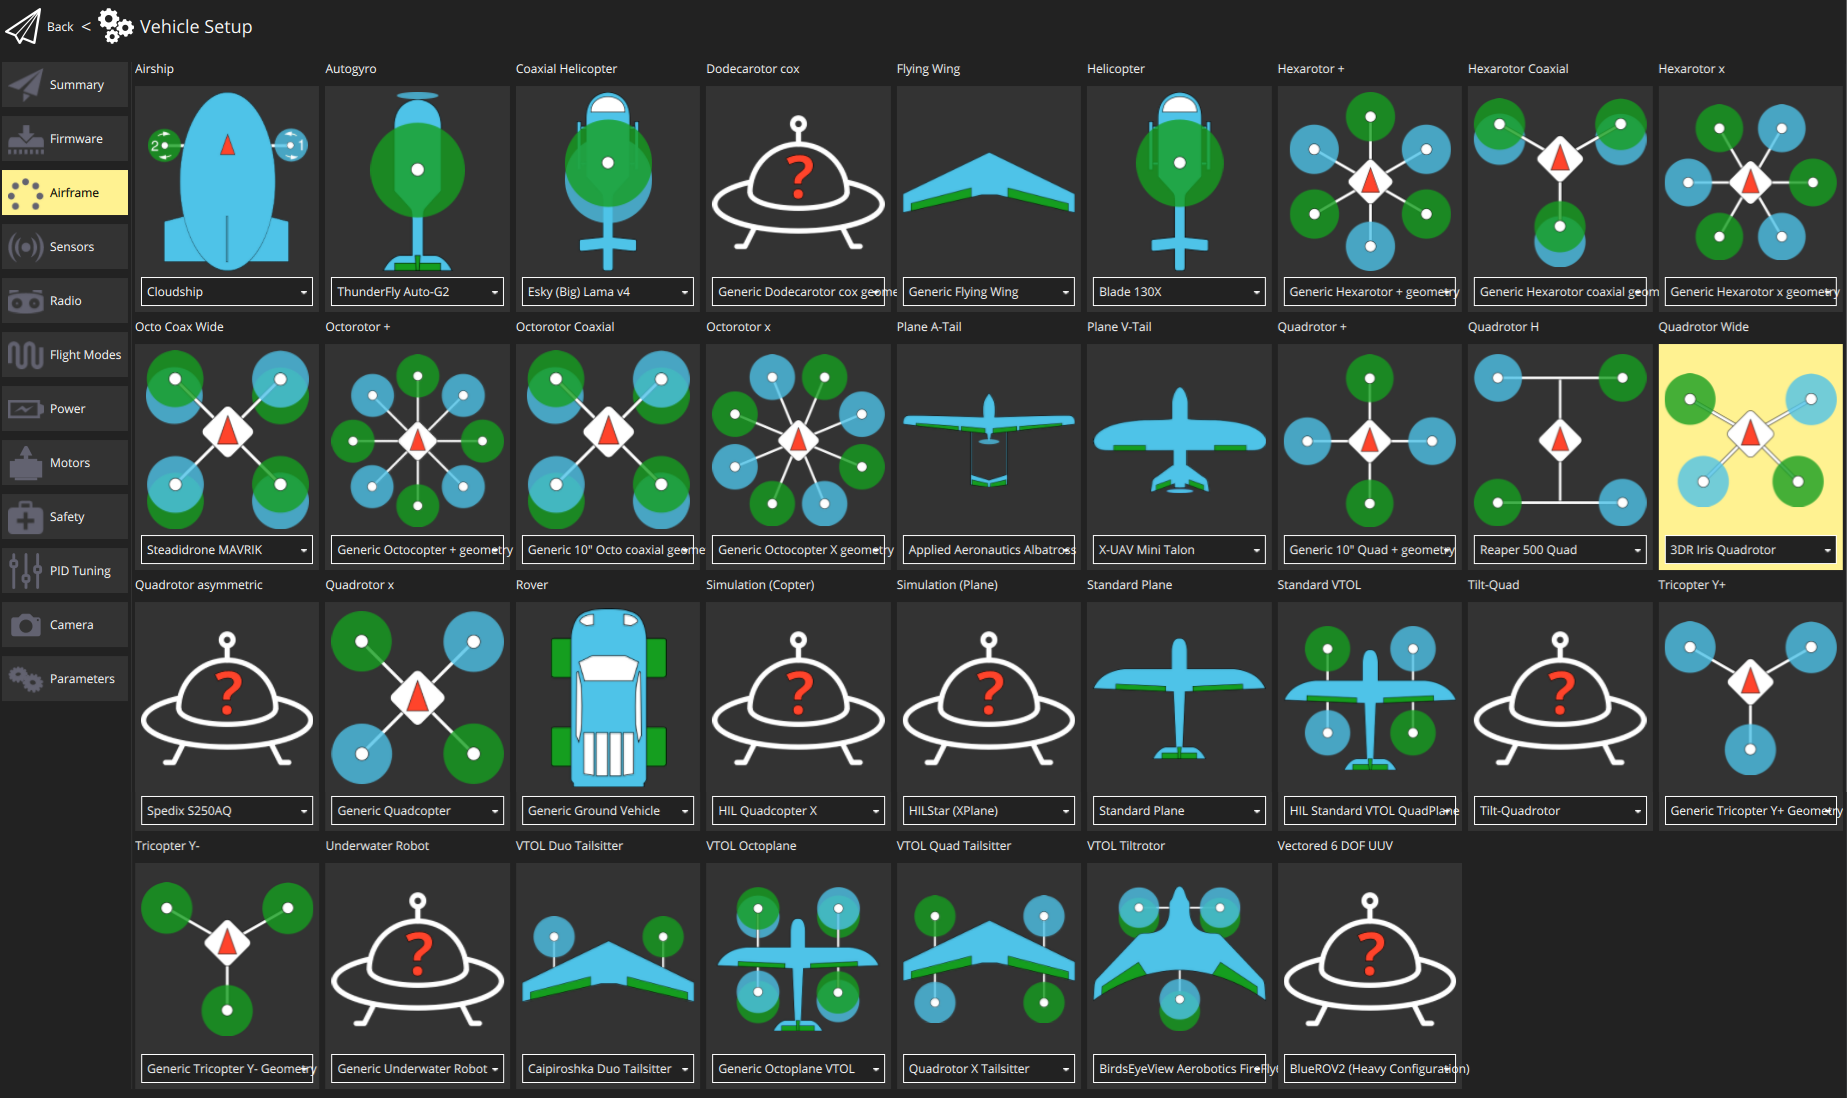
\includegraphics[scale=0.31]{obrazky/QG2}
    \end{center}
    \caption[Základní obrazovka QGroundControl]{Základní obrazovka QGroundControl.}
    \label{fig:QGC1}
\end{figure}

\subsection{Plánování bezpilotní mise}
\label{subs:planovani}

Software QGroundControl nabízí intuitivní plánování bezpilotních misí. Vlastní misi je možné naplánovat pomocí waypointů, nebo pomocí 3 přednastavených plánů pro bezpilotní mise: \cite{QGround2}

\begin{itemize}
    \item Průzkum prostředí
    \item Skenování koridoru
    \item Skenování konstrukcí
\end{itemize}

\subsubsection{Průzkum prostředí}

Pomocí tohoto plánu se vytvoří mřížkový letový vzor nad polygonální oblastí definovanou uživatelem. Oblast je možné definovat jako mnohoúhelník nebo kruh. Je zde taky možné nastavit mřížku přeletů, výšku nad povrchem jako absolutní, nebo relativní vůči terénu. Program umožňuje nastavení snímkování prostředí s podporou geotagging\footnote{Geotagging představuje přidávání geografických metadat k různým médiím jako jsou např.: obrázky.}. Obrázek \ref{fig:QGC2} zobrazuje nastavení autonomní mise s průzkumem prostředí.

\begin{figure}[!ht]
    \begin{center}
        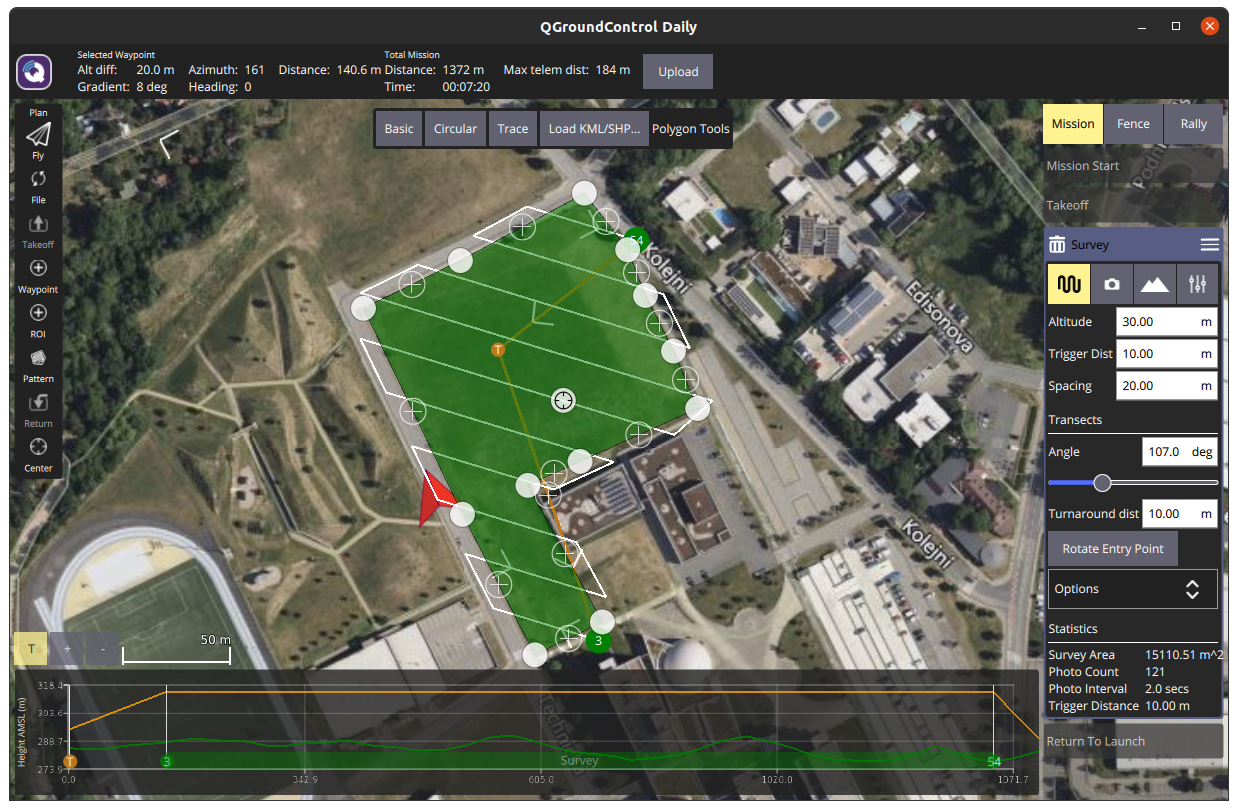
\includegraphics[scale=0.34]{obrazky/QGC3}
    \end{center}
    \caption[Nastavení bezpilotní mise pro průzkum prostředí]{Nastavení bezpilotní mise pro průzkum prostředí.}
    \label{fig:QGC2}
\end{figure}

\subsubsection{Skenování konstrukcí}

Pomocí plánu na skenování konstrukcí je možné naplánovat bezpilotní misi zaměřenou na snímkování svislých povrchů. Snímky se používají na vizuální kontrolu budov, nebo tvorbu 3D modelů konstrukcí. Obrys konstrukce je možné zadat jako mnohoúhelník nebo kruh. Dron bude oblétat celou budovu předem v nastavených výškách tak, aby kamera směřovala vždy na budovu. Po zadání konkrétní kamery, objektivu a rozlišení snímkování [cm/px] si program sám dopočítá vhodnou letovou vzdálenost od budovy a výšku jednotlivých letových vrstev. Na obrázku \ref{fig:QGC3} je zobrazeno nastavení autonomní mise pro skenování konstrukcí.

\begin{figure}[!ht]
    \begin{center}
        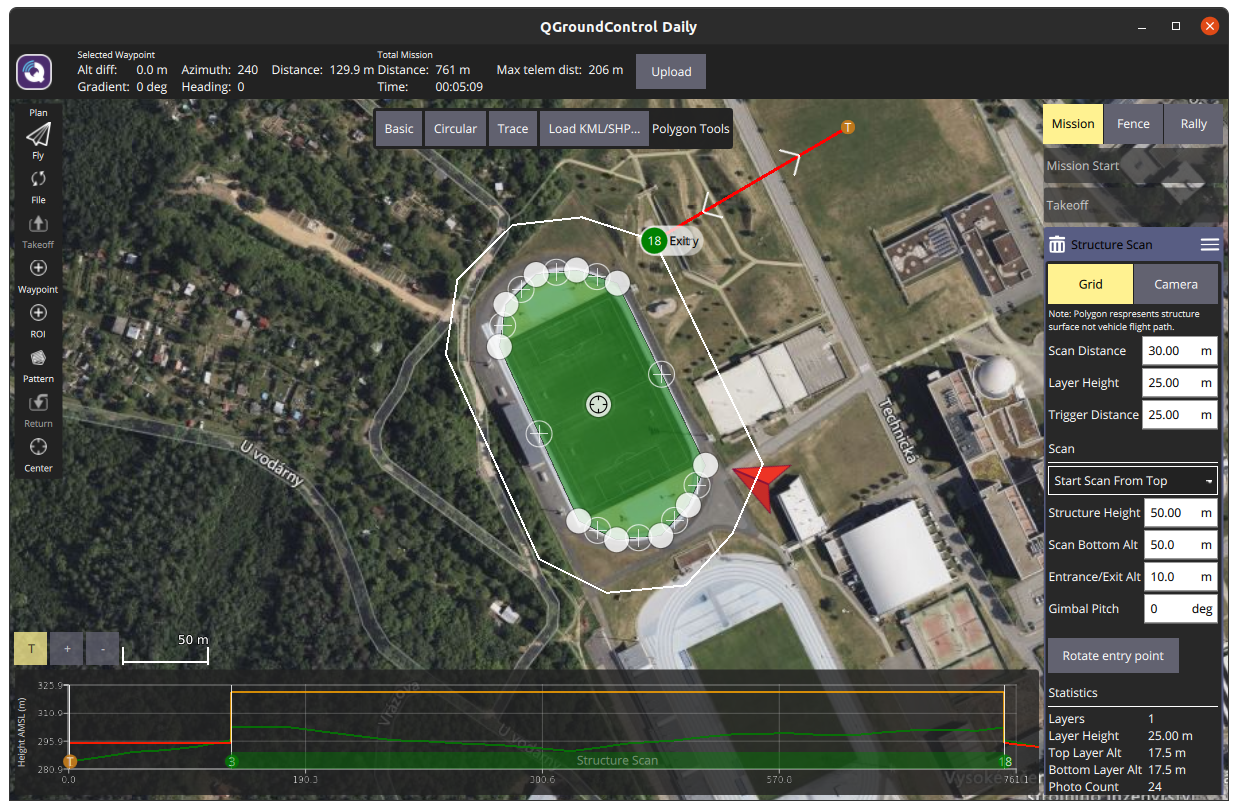
\includegraphics[scale=0.34]{obrazky/QGC5}
    \end{center}
    \caption[Nastavení bezpilotní mise pro skenování konstrukcí]{Nastavení bezpilotní mise pro skenování konstrukcí.}
    \label{fig:QGC3}
\end{figure}

\subsubsection{Skenování koridoru}

Letový plán pro skenování koridoru je vhodný pro sledování křivky (například pro průzkum silnice). Je možné si zde nastavit parametry letového vzoru jako jsou výška přeletu a hustota přeletů nad oblastí. Po zadání parametrů kamery a rozlišení snímkování [cm/px] si program sám dopočítá optimální letový vzor. Obrázek \ref{fig:QGC4} zobrazuje nastavení letového plánu pro skenování koridoru.

\begin{figure}[!ht]
    \begin{center}
        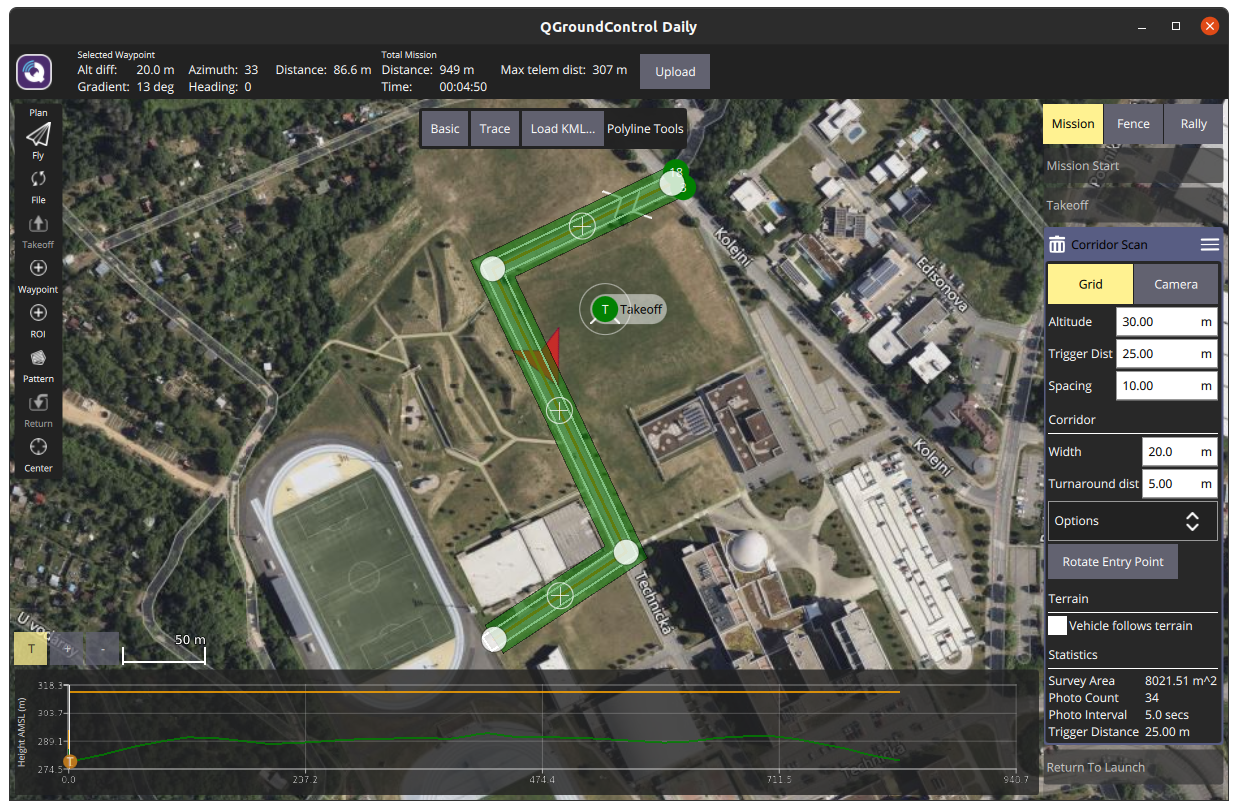
\includegraphics[scale=0.34]{obrazky/QGC4}
    \end{center}
    \caption[Nastavení bezpilotní mise pro skenování koridoru]{Nastavení bezpilotní mise pro skenování koridoru.}
    \label{fig:QGC4}
\end{figure}

